% \commentadd{
% An error in the picking action or the absence of objects exposing top-facing surfaces allowing placement of the object with a single pick, necessitates a strategy to expose a desired pickable surface of the object.
% }
\rahul{
% \begin{figure}
%     \centering
%     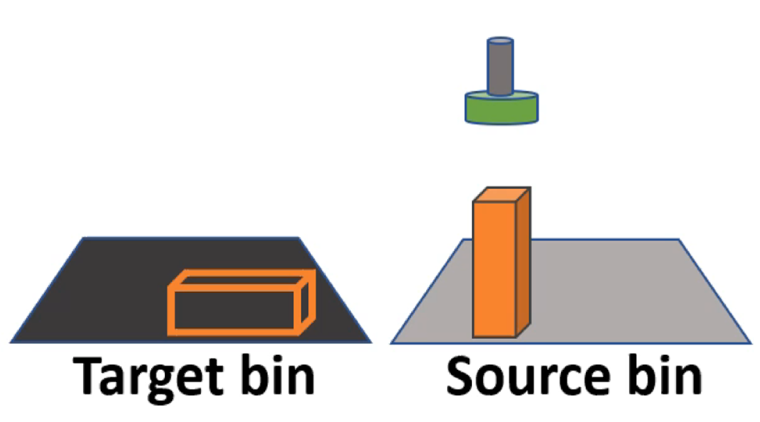
\includegraphics[width=0.3\textwidth]{Figures/toppling_begin.png}
%     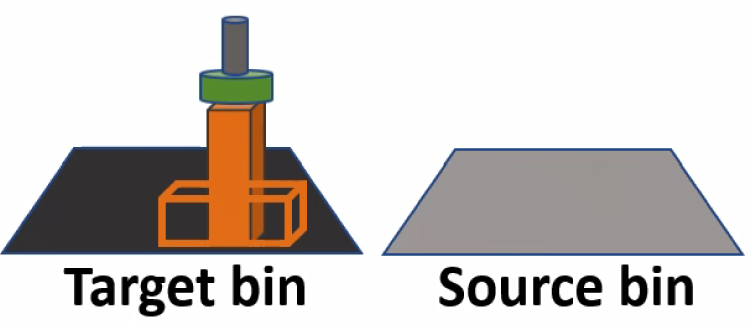
\includegraphics[width=0.3\textwidth]{Figures/toppling_end.png}
%     \caption{An illustration of a scene where a direct pick-and-place fails to solve the problem without reorienting the object. The \textit{top} image shows the initial scene where the orange cuboidal object needs to be transferred to the target bin at the pose denoted by the wireframe marker. The \textit{bottom} image shows the end-effector placing it using a top-down grasp.}
%     \label{fig:reorientation_failure}
% \end{figure}
}
The toppling primitive is invoked if there exists no object that exposes the desirable top-facing surface, or if the object was erroneously picked from the wrong face. The latter is detected after the pick by performing pose estimation once the objet is attached to the suction cup. For instance this can happen for the soaps shown in Figure \ref{fig:pipeline} (right)(d), if the thin side is available for pick but the soap needs to be placed on their wider side. In this case, a toppling primitive is used to reorient the object.
\rahul{
% \begin{figure*}
%     \centering
%     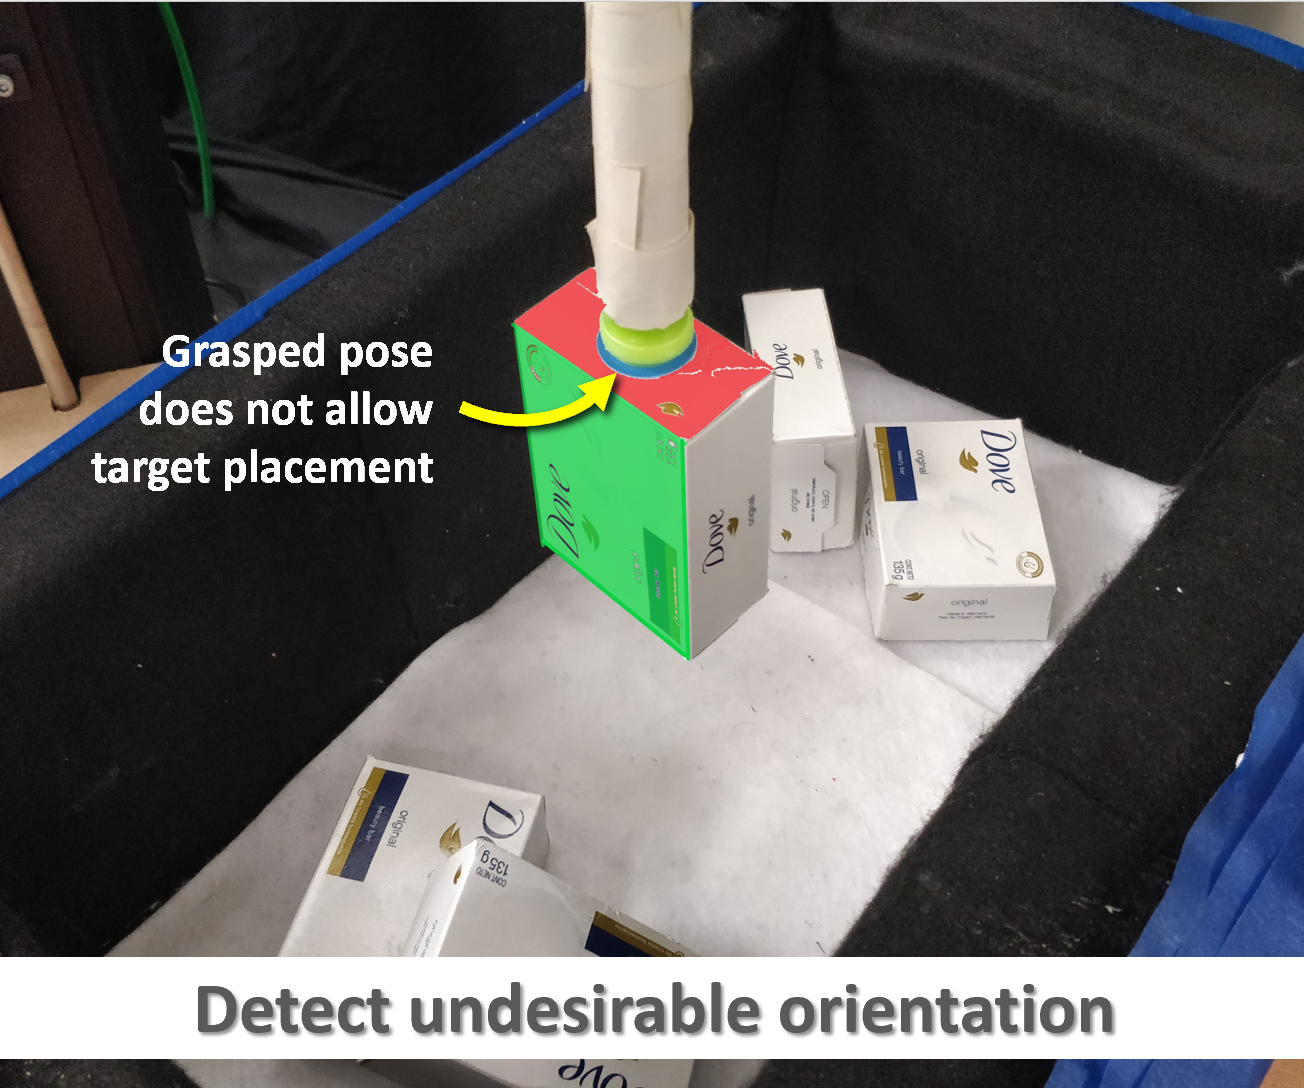
\includegraphics[width=0.24\textwidth]{Figures/toppling1.png}
%     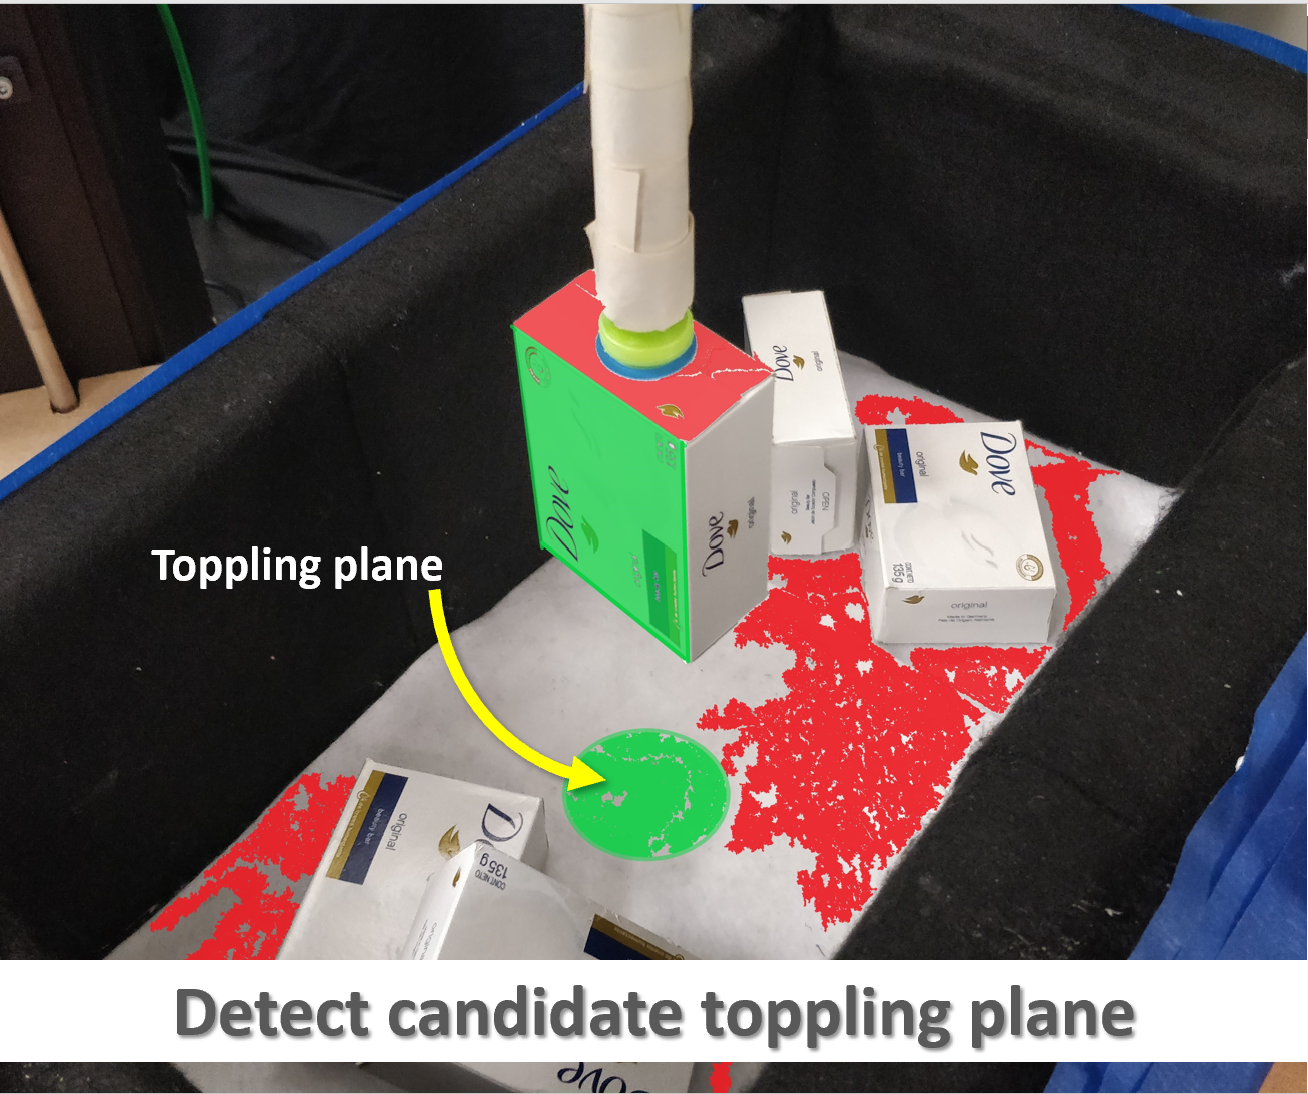
\includegraphics[width=0.24\textwidth]{Figures/toppling2.png}
%     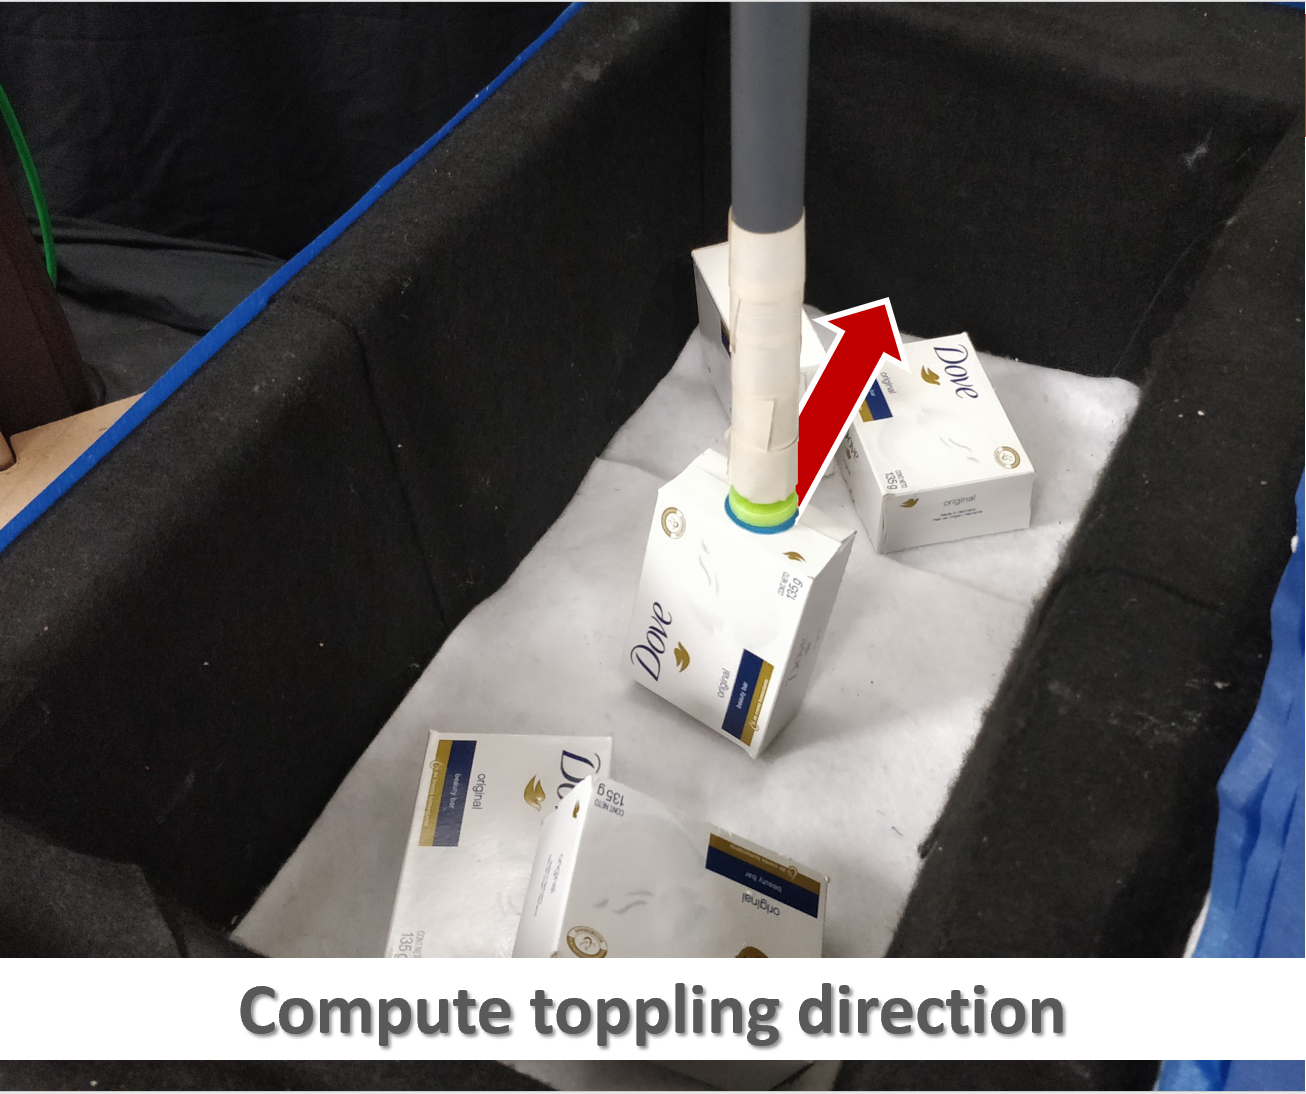
\includegraphics[width=0.24\textwidth]{Figures/toppling3.png}
%     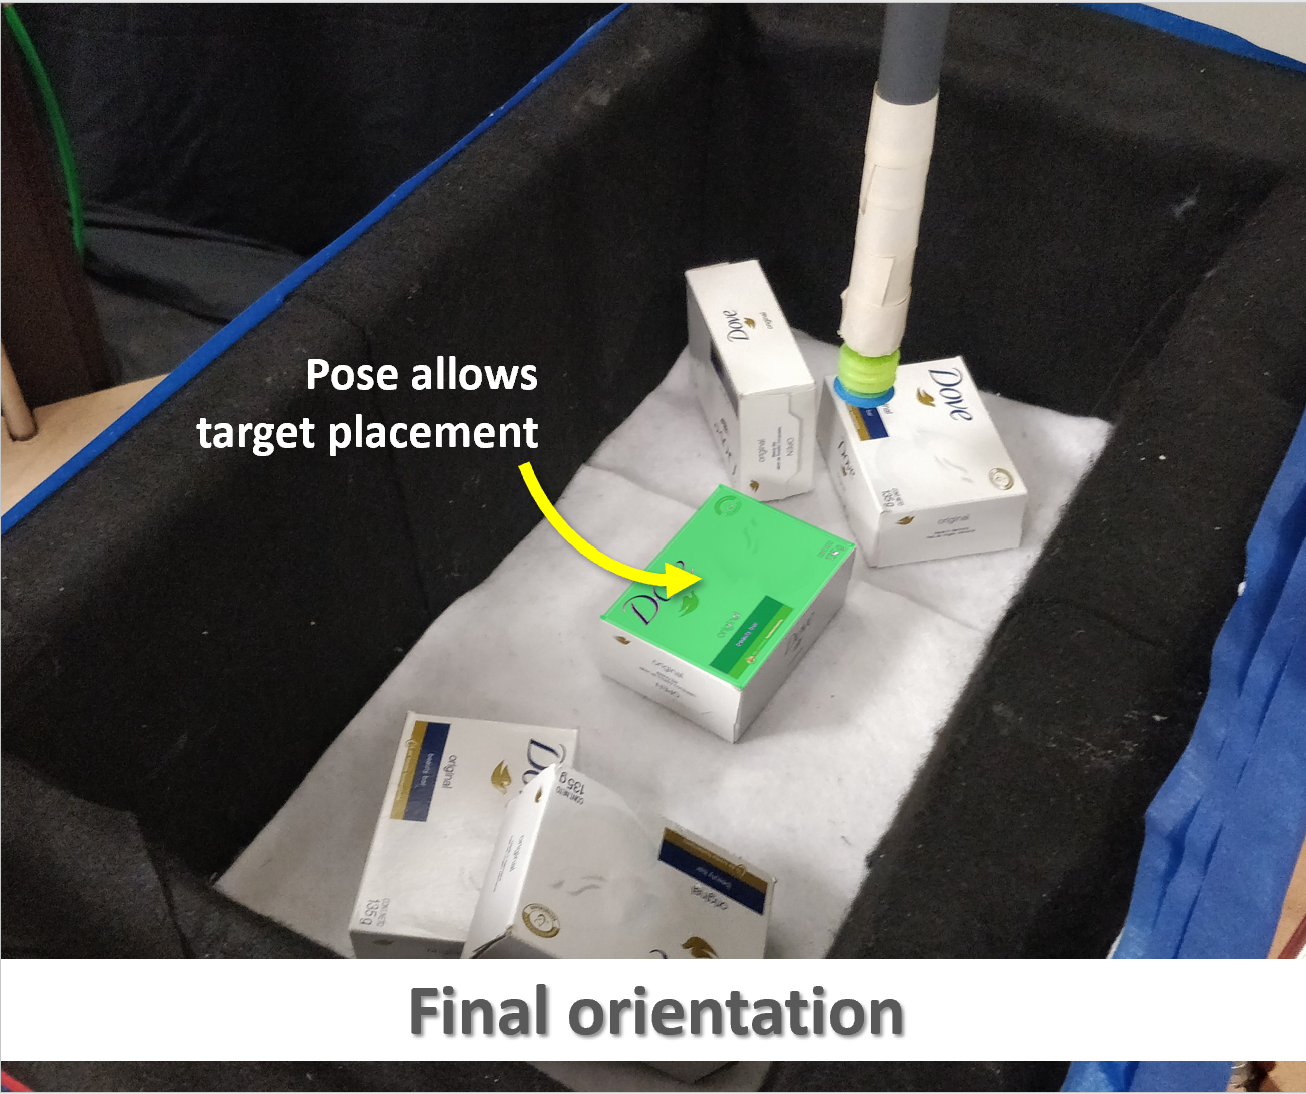
\includegraphics[width=0.24\textwidth]{Figures/toppling4.png}
%     \caption{Steps of toppling primitive from left to right. \textit{Firstly,} the scenario where the grasped pose of the object does not allow the target placement is detected, \textit{secondly,} a plane is detected in the scene that can allow toppling, \textit{thirdly,} the toppling direction is computed and executed, and \textit{finally,} the reoriented object rests in a pose that allows the target placement.}
%     \label{fig:toppling_steps}
% \end{figure*}

\begin{figure*}
    \centering
    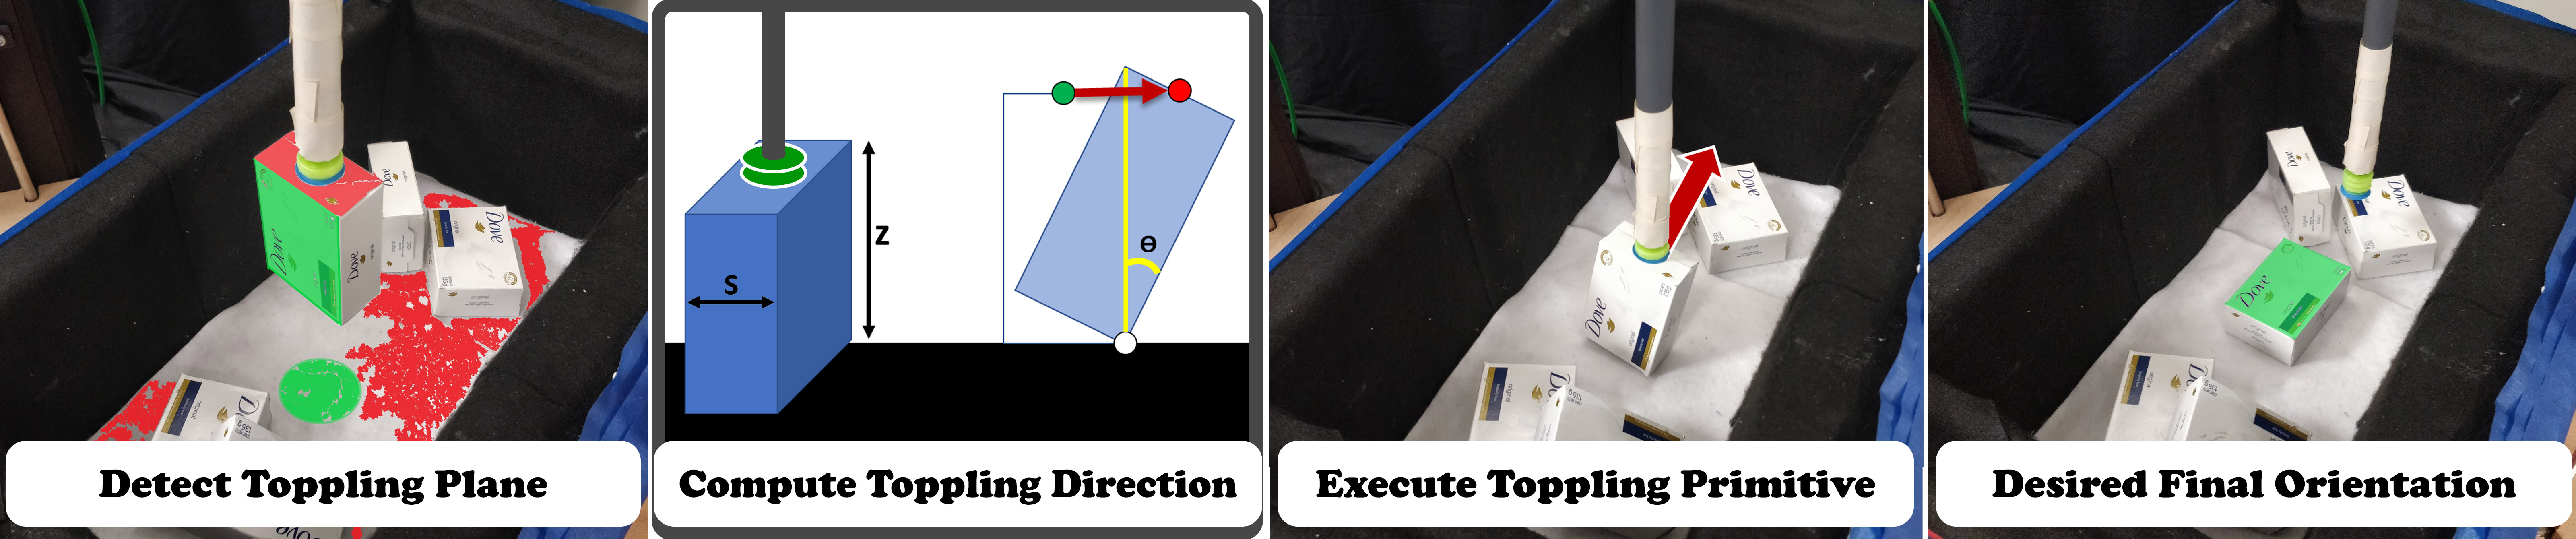
\includegraphics[width=1\textwidth]{Figures/toppling}
    \caption{Steps of toppling primitive from left to right when the scenario where the grasped pose of the object does not allow the target placement is detected. \textit{Firstly,} a plane is detected in the scene that can allow toppling, \textit{secondly,} the toppling direction is computed and \textit{thirdly} executed, and \textit{finally,} the reoriented object rests in a pose that allows the target placement.
    An illustration showing the toppling vector computation with (a) shows the dimensions of the object with \textit{s} being the dimensions along the side that exposes a desired face, and \textit{z} being the height of the top face. On the right, (b) shows the topping vector under the assumption that the object was grasped from the center of the face.
    }
    \label{fig:toppling_steps}
\end{figure*}
}

% The candidate object $o^i$ should be transferred if its detected pose $\pose_{start}$ allows, when moved to $\btarget$, to the next available target pose $\hat{p}^j$. But it could be that while $\graspset( \object^i, \pose_{start} ) \neq \emptyset$, the pose $\pose_{start}$ does not allow the arm to move the object to the target bin in a way that to achieve $\hat{p}^j$. 
% }
% For instance this can happen for the soaps shown in Figure \ref{fig:pipeline} (right), if the thin side is available for pick but the soap needs to be placed on their wider side. 
% In this case, a toppling primitive is used to reorient the object. The toppling primitive is invoked if there exists no object that exposes the desirable picking surface, or if the object was erroneously picked from the wrong face, which is detected after the pick by performing pose estimation on it. 
%Taking into account reachability, collisions and limited symmetry relaxations $\mathbb{P}_{INV}$ can be significantly large enough. A packing method cannot be complete unless there is some explicit reasoning about this set of poses.
%Within the classes of available actions $\{ \mathtt{pick}, \mathtt{release} \}$ a fixed attachment is enforced during a $\mathtt{pick}$, and the constraint is removed during a $\mathtt{release}$. 
% \commentadd{
% Given a starting pose of an object $\pose_{start}$, let the operation $\pose_{topple} = \mathbb{TR}(\pose_{start}, \Pi_{start} )$ represent the pose of the object at the end of the set of actions $\Pi_{topple}: [0,1] \rightarrow \mathcal{X}$ of the arm, defined in the full state space. A toppling action sequence $\Pi_{topple}$ attempts to find a sequence of motions that bring the pose of the object $o^i$ to $\pose_{topple} = \mathbb{TR}(\pose^i, \Pi_{topple} )$, so that:
% % \vspace*{-5mm}
% \begin{equation}
% \exists\ \Pi_{transfer}, \textrm{ so that } D( \mathbb{TR}( \pose_{topple}, \Pi_{transfer} ), \hat{p}^j)  \leq \epsilon
% \label{eq:topple}
% \end{equation}
% }

Given a starting pose of an object $\pose_{start}$ and a toppling action of the arm, the object ends up at a new pose $\pose_{topple}$. The objective is to allow the existence of a pick $\hat{g} \in \graspset( \object^i, \pose_{topple} ) $ so that there is a $\mathtt{transfer}$ action from pick $\hat{g}$ that achieves the final  placement $p_{end}$ close enough to the desired target placement $\hat{p}^j$, i.e., $D(p_{end},\hat{p}^j) \leq \epsilon$. For the considered setup, this means that the top-facing surface of the object at $\pose_{topple}$ and $\hat{p}^j$ is the same.

The toppling module inspects the visible point cloud in the source bin to identify the best toppling plane, which is sufficiently empty and flat. The accompanying implementation restricts actions to ones that change the pose of the cubic objects by shifting the most upward facing surface to only one of the adjacent surfaces. While this does not guarantee toppling the object to all possible poses, the symmetry of cubic products resolves this issue. 

Prior work \cite{lynch1999toppling} has shown the efficacy of minimal end-effectors used in tandem with the environment to achieve toppling. In the previous work, the friction against a conveyor belt is used to topple an object about a resting surface. The conveyor belt's motion is parallel to the initial resting surface plane. In the current setup, the compliance of the suction cup is used to emulate the same effect using a lateral motion on the same plane as the top-surface along the direction of the desired transformation between $\pose_{start}$ and $\pose_{topple}$. Due to symmetry, at least one neighboring surface allows top-down picks, so a successful toppling action exists. Using the pose of the object, the lateral motion direction is executed once the object is placed on the detected plane, and the object is released during this action. Results show that this is highly effective in the target setup.

% of satisfying Eq. \ref{eq:topple}. 

% A high level subroutine in the context of the pipeline is demonstrated as follows.



\rahul{
% \begin{figure}[t]
%     \centering
%     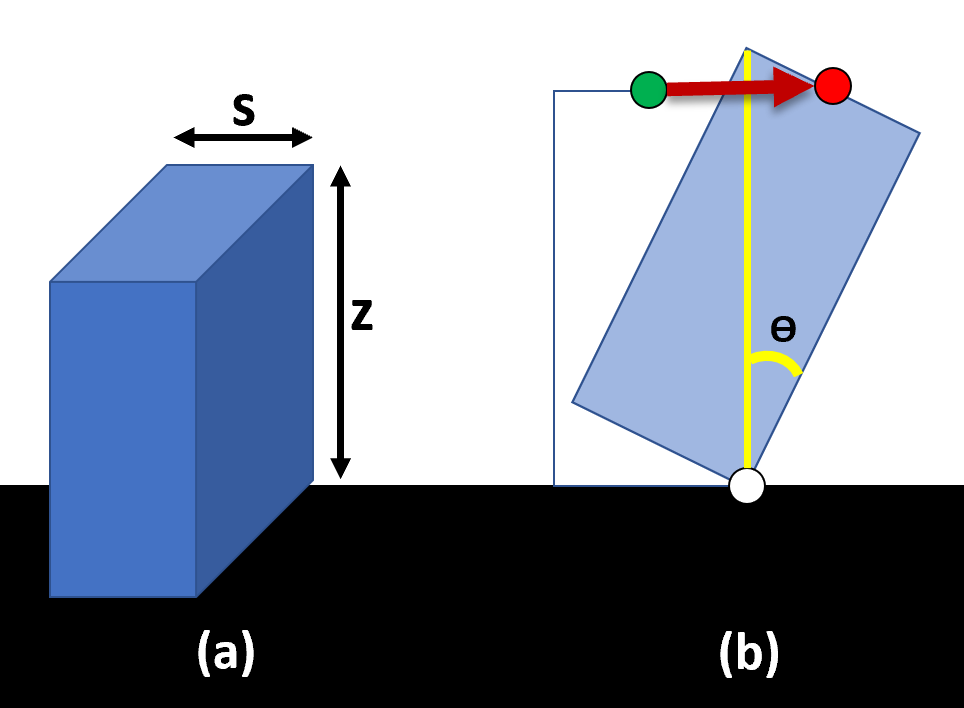
\includegraphics[width=0.48\textwidth]{Figures/toppling_direction.png}
%     \caption{An illustration showing the toppling vector computation with (a) shows the dimensions of the object with \textit{s} being the dimensions along the side that exposes a desired face, and \textit{z} being the height of the top face. On the right, (b) shows the topping vector under the assumption that the object was grasped from the center of the face.}
%     \label{fig:toppling_direction}
% \end{figure}

Algorithm~\ref{algo:topple} describes the high-level sequence of steps involved in executing a toppling action. This subroutine will be invoked once the object is already attached to the end-effector using a top-down grasp, and is also visible to the camera in order to obtain a point cloud. It returns a sequences of poses that constitute the discrete steps of the toppling maneuver, which when executed should drop the object to expose a desired face, denoted by the target orientation.
Line 2 checks whether such a reorientation is even necessary by using the symmetry aware distance between the current grasped pose, and the desired pose. The toppling plane is obtained by estimating a large enough (based on the dimensions of the bottom surface of the object) planar surface on the point cloud, that is also priorized to prefer lower planes than expectedly more unstable higher surfaces on the pile. 

The {\tt GetOffset} primitive is described in Fig~\ref{fig:toppling_steps} (second) to show the computation of the toppling maneuver. Given the pose of the object, the height of the top face is denoted by \textit{z}. Given the desired face(s) that needs to be exposed as the top face to allow the target placement using a top-down grasp, \textit{s} denotes the dimension of the edge(s) not adjacent to the desired face; i.e., out of the two dimensions defining the top-face, select the one that corresponds to the direction of toppling. Define $\theta = \tan^{-1} \frac{s}{z} $. The toppling has to change the orientation of the object till its center (approximating the center of gravity) goes beyond the support point at along the contact edge denoted by the white circle in the image. This object rotation can be affected by displacing the grasp point of contact (green circle) to the {toppled configuration} (red circle). Without loss of generality, consider the point of grasp to be the center of the top face. The offsets become:

\vspace{-0.2in}
$$
	\Delta x = \frac{s}{2} + z \sin \theta - \frac{s}{2} \cos \theta + \epsilon;\ 
	\Delta z = z \cos \theta + \frac{s}{2} \sin \theta - z
$$
\vspace{-0.15in}

Here $\Delta x$ and $\Delta z$ denote the planar and height offsets in the object's local frame describing the toppling vector, shown by the red arrow in Fig~\ref{fig:toppling_steps} (third). $\epsilon$ is meant to allow some error tolerance to the maneuver, when the action is executed by pivoting the object. 

 \begin{algorithm}
 \small
 \DontPrintSemicolon
 \KwIn{Point cloud $C$, object $\object$, top-down current object pose $\pose\gets(t,r)$, target orientation $r_{\mathrm target}$}
 \KwOut{Toppling primitive $\Pi$  }
 	$\Pi\gets\emptyset$;\\
 	\If{ $D$($\pose, (t,r_{\mathrm target}$)) $\ >\ \epsilon $ }
 	{
 		$t_{\mathrm plane} \gets ${\tt GetTopplingPlane}($C, ${\tt Dimensions}($\object$));\\
 		$\pose_{\mathrm plane} \gets (t_{\mathrm plane}, r)$\\
 		$\Pi \gets \Pi \cup \pose_{\mathrm plane}$;\\
 		$(\theta,\Delta x,\Delta z) \gets ${\tt GetOffset}($\object, \pose_{\mathrm plane}, r_{\mathrm target}$);\\
 		$\Pi \gets \Pi \cup $ {\tt ApplyOffset}($\pose_{\mathrm plane}, \theta,\Delta x,\Delta z$);
 	}
 \Return{$\Pi$}
 \caption{{\sc Topple}}
 \label{algo:topple}
 \end{algorithm}

}

% Put ee in image


% There may exist a set of objects in $\objectset$ that require regrasping, because the initial pose of the object $\pose$ in $\ainit$ does not allow any valid grasp that allows a prehensile transfer to the target pose. In such situations, the current solution detects instances where the objects of the source bin are not desirably graspable, raises them above the source bin, tilts and drops them. This maneuver attempts to change the pose of the object to an orthogonal one, which by the nature of symmetry of cuboidal objects, should expose a desirable face to top-down grasps. Once an object's pose is successfully changed to one that allows a transfer to the target bin, the lower levels of the task planning hierarchy can deal with it. 

% Consider an object $\object$ at pose $\pose_{init}$, and $\pose_{goal}$ be the target pose in the context of packing the object in $\btarget$. If it is detected that $\graspset_\object^{\pose_{init}} \cap \graspset_\object^{\pose_{goal}} = \emptyset$, there can be no grasp that can transfer the object. The regrasp task is defined as the sequence of transfers and moves that the object from the initial pose, $\pose_{init} \in \ainit$ to some intermediate pose $\pose_{k}$ at the end of a valid motion of the arm, $\pi_{regrasp}$ such that
% $$
% \pose_k \in \amove_{\pi_{regrasp}}^{\ainit}, \graspset_\object^{\pose_{k}} \cap \graspset_\object^{\pose_{goal}} \neq \emptyset
% $$
% Once the object is at $\pose_k$ a transfer $\pi_T$ can place it in $\pose_{goal}$.
% This operation is applied to all objects in $\objectset$ that require regrasps in order to ensure every object is successfully packed into the target bin. 
